\documentclass[conference]{IEEEtran}
\IEEEoverridecommandlockouts

\usepackage{cite}
\usepackage{amsmath,amssymb,amsfonts}
\usepackage{algorithm}
\usepackage{algorithmic}
\usepackage{graphicx}
\usepackage{booktabs}
\usepackage{array}
\usepackage{textcomp}
\usepackage{xcolor}
\usepackage{url}

\graphicspath{{figures/}{../figures/}}

\begin{document}

\title{Label-Free, Dependency-Aware Channel Selection\\
for Coupled Multi-Channel Sensor Data}

\author{
\IEEEauthorblockN{1\textsuperscript{st} Narek Meloyan}
\IEEEauthorblockA{\textit{Akian College of Science \& Engineering}\\
\textit{American University of Armenia}\\
Yerevan, Armenia}
\and
\IEEEauthorblockN{2\textsuperscript{nd} Aleksandr Hayrapetyan}
\IEEEauthorblockA{\textit{Akian College of Science \& Engineering}\\
\textit{American University of Armenia}\\
Yerevan, Armenia}
\and
\IEEEauthorblockN{3\textsuperscript{rd} Narine Sarvazyan, PhD}
\IEEEauthorblockA{\textit{Orbeli Institute of Physiology of NAS RA}\\
\textit{American University of Armenia}\\
Yerevan, Armenia}
}

\maketitle

\begin{abstract}
A method is presented for selecting a small, informative subset of the original
channels of a multi-channel sensor without the use of any labels. A
group-structured autoencoder is first trained to reconstruct all channels,
yielding a shared latent representation of their joint structure. Each latent
factor is then perturbed, and the change induced in the reconstruction of every
channel is measured; a channel whose reconstruction reacts strongly is one on
which the model relies, which provides a label-free estimate of relevance. A
relevance--redundancy rule converts these estimates into an ordered shortlist of
real channels, so that channels repeating information already retained are
avoided. The same procedure was applied to two markedly different sensing
modalities, with only the front-end encoder altered between them. On a
wearable-sensor activity-recognition benchmark composed of three inertial units
(27 channels), retaining ten channels was found to preserve macro-F1 to within
0.04 of the full set under leave-one-subject-out evaluation, to equal a
supervised mutual-information selector that does use labels, and to be
substantially more stable across subjects than variance ranking. On biomedical
hyperspectral imaging, the same method removed 58--95\% of channels while
classification accuracy was maintained or improved; accuracy rose from 88.2\% to
95.2\% on lichen tissue and from 79.8\% to 85.6\% on a collagen dataset. A single
label-free principle therefore delivers strong, interpretable channel reduction
across very different sensors.
\end{abstract}

\begin{IEEEkeywords}
unsupervised feature selection, channel selection, conditional relevance,
autoencoders, interpretability, human activity recognition, hyperspectral imaging.
\end{IEEEkeywords}

\section{Introduction}
Complex sensors emit many channels that overlap heavily and arrive in natural
groups, such as the three axes of one inertial measurement unit or the emission
bands measured under one excitation in fluorescence imaging. For reasons of cost,
power, transmission bandwidth, and interpretability, only a handful of the actual
channels are often required, rather than a learned mixture of them. The central
difficulty is to determine which channels to keep when no labels are available.

Existing selectors present a trade-off. Unsupervised filters such as variance
ranking or principal component analysis (PCA) score each channel by its own
marginal statistics and disregard how channels depend on one another; as a
consequence, several channels carrying the same information tend to be retained
together. Dependency-aware selectors such as minimum-redundancy
maximum-relevance (mRMR) and joint mutual information (JMI) account for this
redundancy but require labels and density estimation. The region of the design
space that is simultaneously label-free, dependency-aware, and discrete---that
is, returning real channels rather than a projection---remains sparsely
populated.

This paper addresses that region with a method built on a group-structured
autoencoder and perturbation-based attribution, and---more importantly---it is
shown that one such method operates across two very different sensing modalities
by changing only its front-end encoder. The contributions of this work are:
\begin{itemize}
\item A label-free, dependency-aware, and discrete channel selector that combines
a group-structured autoencoder, perturbation-based relevance attribution, and a
relevance--redundancy selection rule;
\item A modality-agnostic selection engine that operates on an abstract layout of
groups, channels, and one regular axis, so that adaptation to a new domain
requires only an encoder matched to that axis;
\item An empirical demonstration that the identical method, evaluated under a
rigorous leave-one-subject-out protocol, matches a supervised selector on
wearable-sensor data without labels and is more stable than variance ranking; and
\item A second verification on biomedical hyperspectral imaging, on which
58--95\% of channels are removed while classification accuracy is maintained or
improved.
\end{itemize}

\section{Background and Related Work}
Channel and feature selection methods are commonly grouped into filter, wrapper,
and embedded families~\cite{ref_lapscore,ref_mcfs}. Filter methods rank channels
by a statistic computed independently of any downstream model. Variance ranking
and PCA are unsupervised but marginal: they ignore inter-channel dependency and
therefore tend to select redundant channels. The Laplacian
score~\cite{ref_lapscore} and multi-cluster feature selection
(MCFS)~\cite{ref_mcfs} introduce manifold structure but remain largely
correlation-based.

Dependency-aware selectors model conditional relevance, the property that a
channel's usefulness depends on which other channels are already retained. mRMR,
JMI, and conditional-mutual-information criteria~\cite{ref_mrmr,ref_jmi} are
effective but supervised, requiring labels and reliable density estimates that
are difficult to obtain for high-dimensional, continuous sensor signals.

Within unsupervised deep learning, the concrete
autoencoder~\cite{ref_concrete} performs differentiable discrete feature
selection through a learned selection layer trained jointly with reconstruction,
and autoencoder-based feature selection~\cite{ref_aefs} uses reconstruction with
sparsity on input weights. In hyperspectral imaging specifically, band selection
has been studied extensively; attention-based networks such as
BS-Net~\cite{ref_bsnet} and a range of search- and clustering-based selectors
rank or cluster spectral bands. The method described here is most closely related
to this lineage. Its distinguishing combination is the use of
\emph{perturbation-based reconstruction sensitivity} as the relevance signal on a
\emph{group-structured} representation, followed by an explicit
relevance--redundancy step, and its demonstrated transfer across modalities.
Table~\ref{tab:positioning} situates the method among representative families.

\begin{table}[t]
\caption{Positioning among representative selector families.}
\label{tab:positioning}
\centering
\footnotesize
\begin{tabular}{@{}lccc@{}}
\toprule
Family & Labels & Models & Returns real \\
(example) & needed & dependency & channels \\
\midrule
Variance / PCA & no & no & yes / no \\
Laplacian, MCFS~\cite{ref_lapscore,ref_mcfs} & no & weak & yes \\
mRMR, JMI~\cite{ref_mrmr,ref_jmi} & yes & yes & yes \\
Concrete AE~\cite{ref_concrete} & no & implicit & yes \\
\textbf{This method} & \textbf{no} & \textbf{yes} & \textbf{yes} \\
\bottomrule
\end{tabular}
\end{table}

\section{Method}
\subsection{Problem Formulation}
A multi-channel observation is organised into $G$ groups. Group $g$ contributes
$C_g$ channels measured over a regular axis (time for sensor streams, space for
images) of length $T$, so that one windowed sample is
$X_g \in \mathbb{R}^{T \times C_g}$ and the full sample is the tuple
$X = (X_1,\dots,X_G)$. The objective is to return an ordered subset
$S \subseteq \{(g,c)\}$ of the original channels, with $|S| = K$, that is
informative and non-redundant, using no labels.

\subsection{Group-Structured Autoencoder}
Each group is encoded independently, and the per-group features are fused by
averaging into a single shared latent representation:
\begin{equation}
z = \frac{1}{G}\sum_{g=1}^{G} E_g(X_g), \qquad
\hat{X}_g = D_g(z),
\end{equation}
where $E_g$ and $D_g$ are the encoder and decoder for group $g$ and
$z \in \mathbb{R}^{d \times T}$ is the fused latent. Averaging (rather than
concatenation) ties the groups into one joint code and keeps the latent size
independent of $G$. Training minimises reconstruction error only, with no labels:
\begin{equation}
\mathcal{L} = \sum_{g=1}^{G}\big\| X_g - D_g(z) \big\|_2^2 .
\end{equation}
The encoder is the only modality-specific component: temporal convolutions are
used for sensor streams and spatial convolutions for images.

\subsection{Perturbation-Based Relevance}
After training, the channels on which the model relies are identified by probing
the latent representation. The most informative latent coordinates are ranked by
their variance across samples, and the top $m$ coordinates are retained. For a
retained coordinate $j$ and a perturbation magnitude $\delta$, the latent is
shifted along that coordinate,
\begin{equation}
z^{(j,\delta)} = z + \delta\, e_j,
\end{equation}
and the resulting change in the reconstruction of every channel is measured and
accumulated. The relevance of channel $c$ in group $g$ is
\begin{equation}
I_{g,c} = \!\!\sum_{j,\delta}\, w_j \,
\frac{1}{NT}\sum_{n,t}
\Big| \big[D_g(z^{(j,\delta)}) - D_g(z)\big]_{n,t,c} \Big|,
\end{equation}
where the average is taken over all samples and axis positions, and $w_j$ weights
each coordinate by its importance. A channel whose reconstruction is sensitive to
the latent factors is one the joint representation depends upon.

\subsection{Normalisation and Relevance--Redundancy Selection}
Because groups may differ in scale, relevances are normalised within each group,
\begin{equation}
\tilde{I}_{g,c} = \frac{I_{g,c}}{\max_{c'} I_{g,c'}},
\end{equation}
which was found to be preferable to dividing by the data variance when the
discriminative channels themselves have high variance. Channels are then chosen
by a maximal-marginal-relevance rule that balances relevance against redundancy
with respect to already-selected channels:
\begin{equation}
c^\star = \arg\max_{(g,c)\notin S}
\Big[\, \tilde{I}_{g,c} - \lambda \max_{s\in S}\, \mathrm{sim}\big((g,c), s\big) \Big],
\end{equation}
where $\mathrm{sim}$ is the cosine similarity between the channels' data
profiles and $\lambda$ controls the redundancy penalty. Selection begins with the
most relevant channel and proceeds greedily, yielding an ordered list that can be
truncated to any budget $K$. The complete procedure is given in
Algorithm~\ref{alg:select} and summarised in Fig.~\ref{fig:method}.

\begin{algorithm}[t]
\caption{Label-free dependency-aware channel selection}
\label{alg:select}
\begin{algorithmic}[1]
\STATE \textbf{Input:} grouped data $X=(X_1,\dots,X_G)$, budget $K$,
weight $\lambda$
\STATE Train $\{E_g,D_g\}$ to minimise $\mathcal{L}$ (no labels)
\STATE Compute latent $z$ and rank coordinates by variance; keep top $m$
\FORALL{retained coordinate $j$ and magnitude $\delta$}
  \STATE Form $z^{(j,\delta)}=z+\delta e_j$; accumulate $I_{g,c}$ via Eq.~(4)
\ENDFOR
\STATE Normalise within each group: $\tilde I_{g,c}$ via Eq.~(5)
\STATE $S \leftarrow \{\arg\max_{(g,c)} \tilde I_{g,c}\}$
\WHILE{$|S| < K$}
  \STATE $c^\star \leftarrow$ Eq.~(6); \quad $S \leftarrow S \cup \{c^\star\}$
\ENDWHILE
\STATE \textbf{return} ordered subset $S$
\end{algorithmic}
\end{algorithm}

\begin{figure*}[t]
\centering
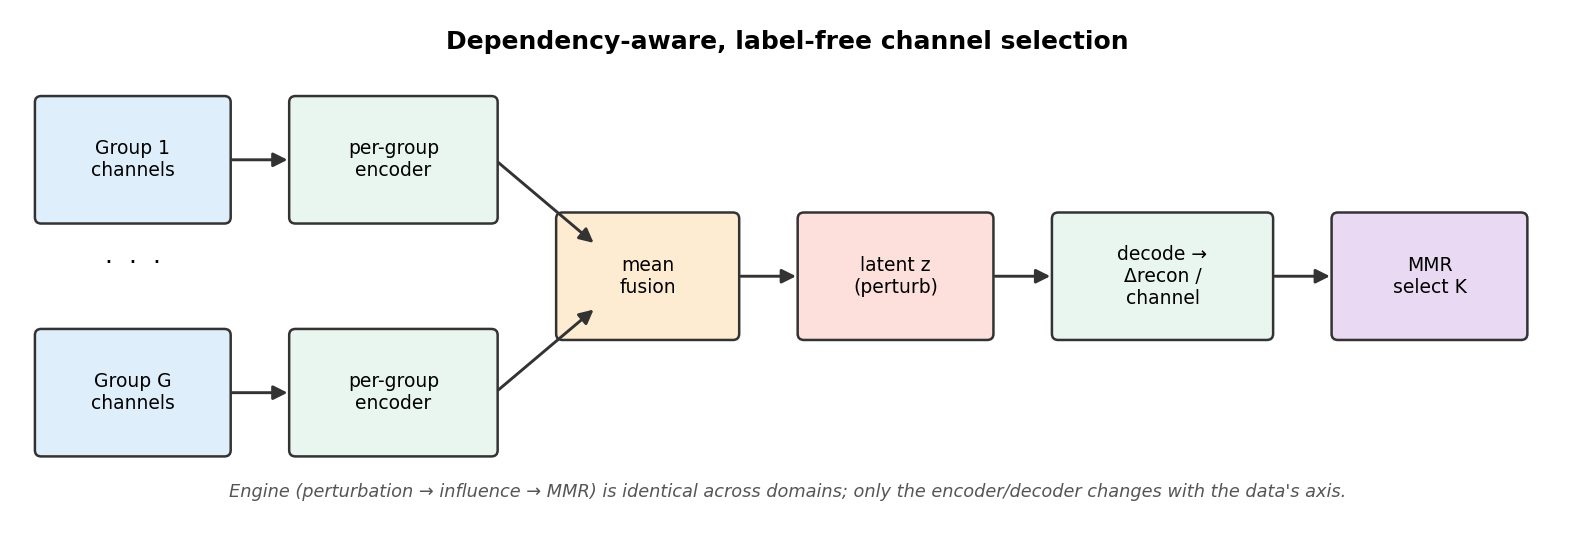
\includegraphics[width=0.92\textwidth]{fig_method.png}
\caption{The three-stage pipeline. A group-structured autoencoder is trained by
reconstruction; latent perturbations yield a per-channel relevance; and a
relevance--redundancy rule selects an ordered subset. The selection engine is
identical across domains; only the encoder and decoder change to match the data's
regular axis.}
\label{fig:method}
\end{figure*}

\subsection{Cross-Domain Instantiation}
The selection engine never accesses raw modality-specific structure; it operates
only on groups, channels, and the latent. Consequently, the same engine is
instantiated in two domains by substituting the encoder
(Fig.~\ref{fig:crossdomain}). For wearable sensors, a group is a body-worn
inertial unit, a channel is one sensor axis, the regular axis is time, and a
one-dimensional convolutional encoder is used. For fluorescence hyperspectral
imaging, a group is an excitation wavelength, a channel is an emission band, the
regular axis is the two-dimensional image plane, and a spatial convolutional
encoder is used.

\begin{figure*}[t]
\centering

\includegraphics[width=0.92\textwidth]{fig_crossdomain.png}
\caption{One method, two verification domains. Only the encoder changes;
the groups--channels--axis abstraction and the selection engine are shared.}
\label{fig:crossdomain}
\end{figure*}

\section{Experimental Setup}
\subsection{Datasets}
Two sensing modalities were used, summarised in Table~\ref{tab:datasets}. The
wearable-sensor dataset was PAMAP2, recorded from three inertial measurement
units (IMUs) placed on the hand, chest, and ankle at 100~Hz. Each IMU contributes
nine channels (three-axis accelerometer, gyroscope, and magnetometer), giving 27
channels organised into three natural groups. A preprocessed release with fixed
one-second windows was used, yielding 38{,}856 windows across eight subjects and
twelve activity classes. The biomedical modality consisted of multi-excitation
fluorescence hyperspectral image cubes: a lichen-tissue dataset (eight
excitations, 192 emission bands, four classes) and a collagen dataset (six
excitations, 158 bands, three classes).

\begin{table}[t]
\caption{Datasets used for verification.}
\label{tab:datasets}
\centering
\footnotesize
\begin{tabular}{@{}lccccc@{}}
\toprule
Dataset & Modality & Groups & Channels & Classes & Axis \\
\midrule
PAMAP2 & IMU & 3 & 27 & 12 & time \\
Lichens & HSI & 8 & 192 & 4 & space \\
Collagen & HSI & 6 & 158 & 3 & space \\
\bottomrule
\end{tabular}
\end{table}

\subsection{Implementation Details}
For the wearable-sensor encoder, each group was processed by a stack of
one-dimensional convolutions over time (kernel size five) producing a latent of
dimension sixteen, with a mirrored decoder; for the imaging encoder, spatial
convolutions were used in place of temporal ones. Networks were trained by the
Adam optimiser for a small number of epochs on the reconstruction objective,
without any labels. During attribution, the top forty latent coordinates by
variance were perturbed at two magnitudes, and relevances were accumulated as in
Eq.~(4). The redundancy weight was set to $\lambda = 0.5$, and similarity was
computed as the cosine similarity between channel data profiles. All computation
was performed on a single workstation; no dataset-specific tuning of the selector
was applied beyond the per-group normalisation described above.

\subsection{Protocol}
For the wearable-sensor data, a strict leave-one-subject-out (LOSO) protocol was
used: for each held-out subject, the autoencoder was trained without labels on
the remaining subjects' windows, the selection engine produced an ordered channel
list, and the chosen subset was then verified by training a $k$-nearest-neighbour
classifier ($k{=}5$) on those channels and measuring macro-F1 on the held-out
subject. All reported values are LOSO means. The label-free selector was compared
against a supervised mutual-information selector, an unsupervised variance
baseline, and random selection. For the hyperspectral data, the identical
selection engine was applied with a spatial encoder, and per-pixel
classification accuracy was used for verification.

\section{Results and Discussion}
\subsection{Wearable-Sensor Activity Recognition}
The relationship between the number of retained channels and recognition
performance is shown in Fig.~\ref{fig:acck} and Table~\ref{tab:har}. Reducing
from 27 to 10 channels (a 63\% reduction) was found to preserve macro-F1 to
within 0.04 of the full-set value. Across channel budgets, the label-free method
tracked the supervised mutual-information selector and remained above the variance
baseline. The selected channels were also more stable across subjects
(Fig.~\ref{fig:stability}): variance selection varied widely from subject to
subject, whereas the proposed method did not, which is important when a single
sensor set must be fixed before deployment. A representative selection
(Fig.~\ref{fig:harsel}) was distributed across all three body locations and
across accelerometer, gyroscope, and magnetometer channels, indicating that a
diverse, interpretable subset was obtained rather than several copies of one
strong signal.

\begin{table}[t]
\caption{HAR macro-F1 under channel reduction (LOSO). Full set (27~ch) $=0.72$.}
\label{tab:har}
\centering
\footnotesize
\begin{tabular}{@{}lccc@{}}
\toprule
Method & 10~ch ($-63\%$) & 7~ch ($-74\%$) & 5~ch ($-81\%$) \\
\midrule
This method (label-free) & \textbf{0.68} & \textbf{0.63} & 0.54 \\
Mutual info (supervised) & 0.68 & 0.61 & 0.54 \\
Variance (unsupervised)  & 0.59 & 0.54 & 0.51 \\
\bottomrule
\end{tabular}
\end{table}

\begin{figure}[t]
\centering
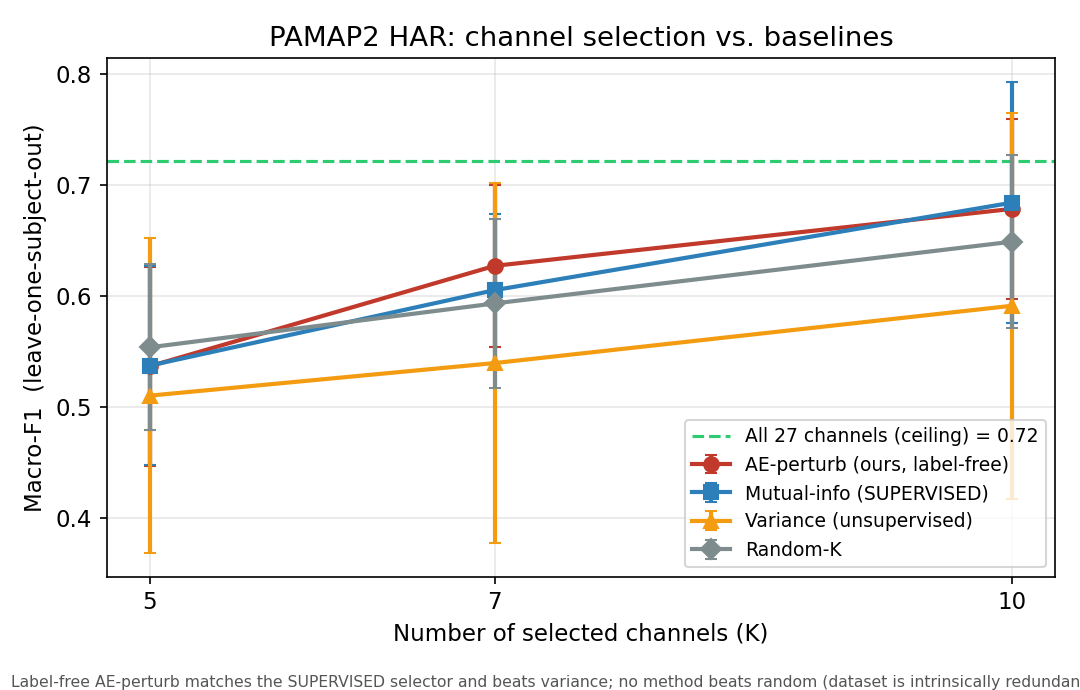
\includegraphics[width=\linewidth]{fig_acc_vs_k.png}
\caption{Macro-F1 versus number of retained channels (LOSO). The label-free
method (red) tracks the supervised selector (blue) and stays above variance
(orange); the dashed line is the full-set ceiling.}
\label{fig:acck}
\end{figure}

\begin{figure}[t]
\centering
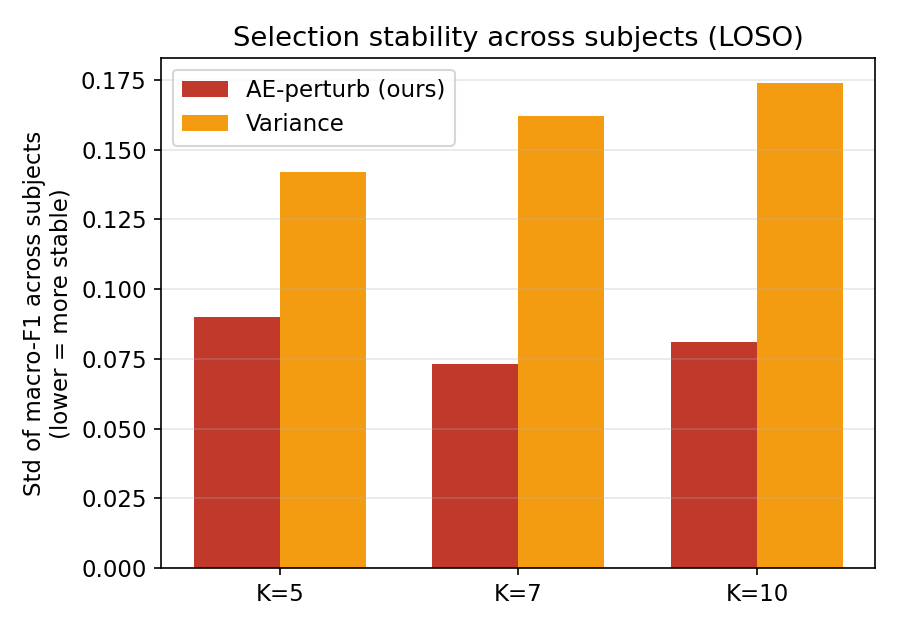
\includegraphics[width=\linewidth]{fig_stability.png}
\caption{Stability of the selected set across subjects (lower is better). The
proposed method is markedly more consistent than variance selection.}
\label{fig:stability}
\end{figure}

\begin{figure}[t]
\centering
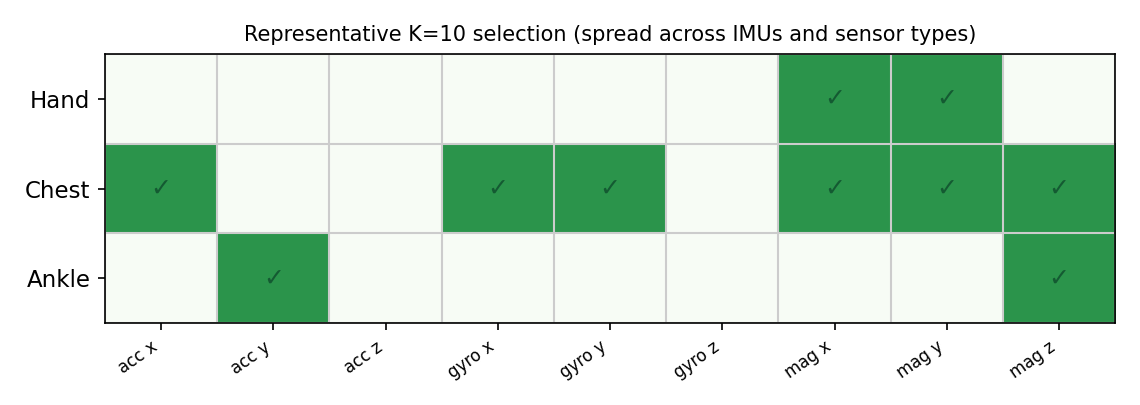
\includegraphics[width=\linewidth]{fig_har_selection.png}
\caption{A representative ten-channel selection, distributed across the three
inertial units and across sensor types.}
\label{fig:harsel}
\end{figure}

For full transparency, it was observed that on this particular benchmark no
selector, including the supervised one, surpassed random selection. The 27
channels are highly redundant, so almost any moderate subset approaches the
full-set ceiling; this property was confirmed by the supervised
mutual-information selector also failing to separate from random. The informative
comparisons on this dataset are therefore the agreement with a supervised
selector obtained without labels and the improvement in stability over variance.

\subsection{Biomedical Hyperspectral Imaging}
The identical method was verified on biomedical fluorescence hyperspectral
imaging, where the redundancy among bands is high and intelligent selection is
expected to separate clearly from trivial baselines. On the lichen-tissue
dataset, 95.2\% classification accuracy was reached using 80 of 192 bands, above
the 88.2\% obtained with all bands, and 89.4\% was still achieved using only nine
bands (a 95\% reduction). On the collagen dataset, 30 bands raised accuracy from
79.8\% to 85.6\%. These results are summarised in Table~\ref{tab:biomed} and
Fig.~\ref{fig:biomed}, and they complement the wearable-sensor result by showing
that, in a high-redundancy regime, the same selection principle yields large
reductions with no loss---and often a gain---in accuracy.

\begin{table}[t]
\caption{Biomedical HSI: aggressive reduction maintains or improves accuracy.}
\label{tab:biomed}
\centering
\footnotesize
\begin{tabular}{@{}lccc@{}}
\toprule
Dataset & Channels (all\,$\rightarrow$\,kept) & Reduction & Accuracy \\
\midrule
Lichens  & $192 \rightarrow 80$ & 58\% & $88.2 \rightarrow 95.2\%$ \\
Lichens  & $192 \rightarrow 9$  & 95\% & $88.2 \rightarrow 89.4\%$ \\
Collagen & $158 \rightarrow 30$ & 81\% & $79.8 \rightarrow 85.6\%$ \\
\bottomrule
\end{tabular}
\end{table}

\begin{figure}[t]
\centering
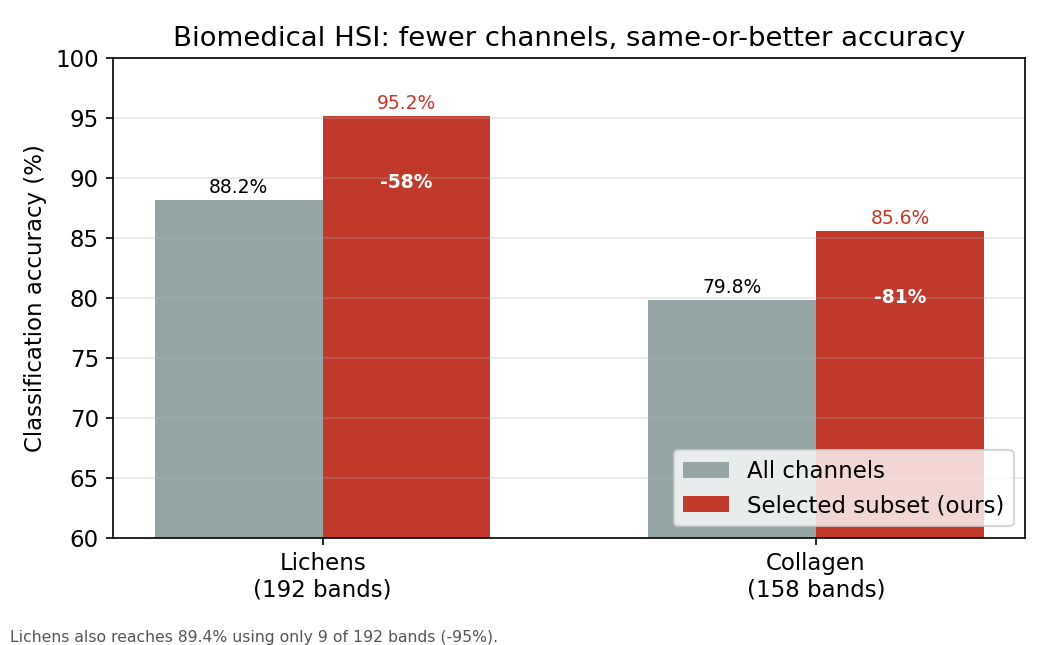
\includegraphics[width=\linewidth]{fig_biomed.png}
\caption{Biomedical hyperspectral imaging: fewer channels, same-or-better
accuracy. Lichens additionally reaches 89.4\% using only nine of 192 bands.}
\label{fig:biomed}
\end{figure}

\subsection{Discussion}
Two observations follow from the experiments. First, the value of a channel
selector depends strongly on the redundancy of the dataset. On a saturated
benchmark such as PAMAP2, where the channels are highly correlated, even a
supervised selector cannot exceed random selection, and the meaningful axes of
comparison become agreement with supervised methods and stability. On a
high-redundancy imaging regime, the same method removes most channels with no
loss of accuracy. Second, modelling redundancy explicitly is what separates the
proposed method from variance ranking: variance repeatedly selects high-variance
but mutually redundant channels, whereas the relevance--redundancy rule spreads
the budget across complementary channels, which also explains the improved
stability across subjects.

\subsection{Computational Considerations}
The cost of the method is dominated by the unsupervised training of the
group-structured autoencoder, which is performed once per training split. The
attribution stage requires one decoder pass for each retained latent coordinate
and perturbation magnitude, and is therefore linear in the number of probed
coordinates; with a few tens of coordinates this stage is inexpensive relative to
training. The relevance--redundancy selection operates on the compact
$(\text{group},\text{channel})$ catalogue and is negligible. Because selection is
unsupervised and performed once, its cost is amortised over all subsequent uses of
the reduced channel set, and at deployment only the selected channels need be
acquired and processed.

\subsection{Limitations}
The benefit of selection is bounded by the redundancy of the data. On strongly
redundant benchmarks, no selector---supervised or unsupervised---can be expected
to exceed random selection by a wide margin, and comparisons should emphasise
agreement with supervised methods and selection stability rather than absolute
gains over random. The method also assumes a meaningful grouping of channels;
where no natural grouping exists, a single group may be used at the cost of the
dependency structure that the group fusion is designed to exploit.

\section{Conclusion}
A single unsupervised, dependency-aware selection principle was shown to deliver
strong, interpretable channel reduction across two very different modalities,
requiring only a change of encoder. On wearable sensors it matched a supervised
selector without labels and selected more stably than variance ranking; on
biomedical imaging it removed 58--95\% of channels while accuracy was maintained
or improved. Future work will target a higher-redundancy activity benchmark, on
which selection is expected to separate from random by a wide margin, and a
direct comparison with differentiable unsupervised selectors such as the concrete
autoencoder.

\section*{Acknowledgment}
The authors thank the AUA Akian College of Science \& Engineering for
institutional support and the L.A. Orbeli Institute of Physiology, NAS RA. AI
assisted tools were used during the preparation of this paper for code
scaffolding, figure generation, and language refinement; all experimental design,
analysis, results, and conclusions are the authors' own work and were verified by
the authors.

\begin{thebibliography}{00}
\bibitem{ref_concrete} M. F. Bal\i{}n, A. Abid, and J. Zou, ``Concrete
autoencoders: Differentiable feature selection and reconstruction,'' in
\emph{Proc. ICML}, 2019.
\bibitem{ref_mrmr} H. Peng, F. Long, and C. Ding, ``Feature selection based on
mutual information: Criteria of max-dependency, max-relevance, and
min-redundancy,'' \emph{IEEE Trans. Pattern Anal. Mach. Intell.}, vol.~27,
no.~8, pp.~1226--1238, 2005.
\bibitem{ref_jmi} G. Brown, A. Pocock, M.-J. Zhao, and M. Luj\'an, ``Conditional
likelihood maximisation: A unifying framework for information theoretic feature
selection,'' \emph{J. Mach. Learn. Res.}, vol.~13, pp.~27--66, 2012.
\bibitem{ref_lapscore} X. He, D. Cai, and P. Niyogi, ``Laplacian score for
feature selection,'' in \emph{Proc. NeurIPS}, 2005.
\bibitem{ref_mcfs} D. Cai, C. Zhang, and X. He, ``Unsupervised feature selection
for multi-cluster data,'' in \emph{Proc. ACM SIGKDD}, 2010, pp.~333--342.
\bibitem{ref_aefs} K. Han, Y. Wang, C. Zhang, C. Li, and C. Xu, ``Autoencoder
inspired unsupervised feature selection,'' in \emph{Proc. IEEE ICASSP}, 2018,
pp.~2941--2945.
\bibitem{ref_bsnet} Y. Cai, X. Liu, and Z. Cai, ``BS-Nets: An end-to-end
framework for band selection of hyperspectral image,'' \emph{IEEE Trans. Geosci.
Remote Sens.}, vol.~58, no.~3, pp.~1969--1984, 2020.
\bibitem{ref_pamap2} A. Reiss and D. Stricker, ``Introducing a new benchmarked
dataset for activity monitoring,'' in \emph{Proc. IEEE Int. Symp. Wearable
Computers (ISWC)}, 2012, pp.~108--109.
\bibitem{ref_monster} A. Dempster et al., ``MONSTER: Monash scalable time series
evaluation repository,'' arXiv:2502.15122, 2025.
\bibitem{ref_knn} T. Cover and P. Hart, ``Nearest neighbor pattern
classification,'' \emph{IEEE Trans. Inf. Theory}, vol.~13, no.~1, pp.~21--27,
1967.
\end{thebibliography}

\end{document}
